\documentclass[a4paper]{article}
\usepackage[spanish]{babel}
\usepackage{hyperref}
\usepackage{graphicx}
\usepackage{fancyhdr}
\usepackage[margin=3.5cm, top=2.5cm, bottom=3cm, includefoot]{geometry}
\usepackage{xcolor}


\graphicspath{ {imagenes1/} }

\setlength{\headsep}{2.5cm}
\pagestyle{fancy}
\fancyhf{}
\lhead{
\includegraphics[width=4cm]{Nuevo-Logo-1.jpg}}
\rfoot{{\textbf{Spark} \\ Master en Big Data y Data Science}}
\lfoot{ \break Página \thepage}
\renewcommand{\headrulewidth}{0pt}





\begin{document}
\begin{titlepage}
    \centering
    {\bfseries\LARGE Universidad Internacional de Valencia \par}
    \vspace{1cm}
    {\scshape\Large Master en Big Data y Data Science \par}
    \vspace{3cm}
    {\scshape\Huge Problema 1: Gasto sin tarjeta de crédito \par}
    \vspace{1cm}
    \begin{figure}[h]
        \centering
        
\includegraphics[width=8cm, keepaspectratio]{Nuevo-Logo-1.jpg}

    \end{figure}
    \vspace{1cm}
    {\itshape\Large Procesamiento de datos masivos: Spark \par}
    \vspace{3cm}
    {\Large Autor: \par}
    {\Large Adrián Hernández Padrón \par}
    {\Large Julio 2022 \par}


\end{titlepage}
\clearpage
\begin{section}{Código}  
    Para empezar tenemos que leer los datos de entrada, esto lo hacemos iniciando la sesión del programa e indicandole la ruta del archivo
    con los datos la cual hemos guardado en la variable entrada.
    \begin{figure}[h]
        \centering
        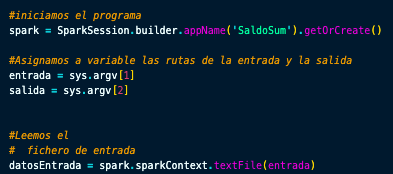
\includegraphics[width=\textwidth, keepaspectratio]{codigo1}
        \caption{Con este código ya hemos cargado los datos de entrada guardados en el fichero entrada1.txt}
    \end{figure}
    Entonces ya podemos trabajar con estos datos, el primer paso dentro de la función será crear una variable vacía, que en este caso llamamos clavevalor, donde guardaremos la respuesta del map y separar las lineas haciendo uso del .split() separando por el salto de línea.
    De esta manera en la nueva variable, new\_linea, la información estará ya separada por filas. Cuando ejecutamos el bucle for, vamos recorriendo fila por fila y separando nuevamente entre el nombre, metodo y salto y guardamos nuestros pares clave-valor.
    \begin{figure}[h]
        \centering
        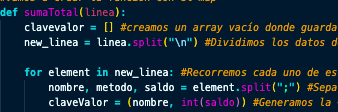
\includegraphics[width=\textwidth, keepaspectratio]{codigo2}
        \caption{Vemos como guardamos nuestros pares clave-valor(saldo(str)-valor(int) los cuales serán la salida del ejercicio.)}
    \end{figure}
    
    Ya lo último que nos queda hacer dentro del map es separar la información según el método de pago, esto se hace con un if-else. Dentro del else, tratamos el caso de una persona que haya comprado unicamente con tarjeta de crédito.
    \begin{figure}[h]
        \centering
        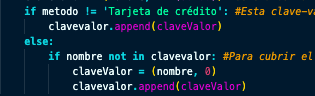
\includegraphics[width=\textwidth, keepaspectratio]{codigo3}
        \caption{Dentro del else realizamos un if que agregará (Nombre,0) en caso de que el nombre no se encuentre en la variable de salida.}
    \end{figure}
    Con esto ya preparamos la salida de los datos del map, correctamente clasificados. Lo que queda ahora es sumar estos datos, esto lo hacemos haciendo uso del reduceByKey sobre la siguiente función.
    \begin{figure}[h]
        \centering
        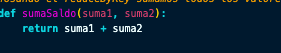
\includegraphics[width=\textwidth, keepaspectratio]{codigo4}
        \caption{Función que ejecuta el reduceByKey para poder sumar todos los gastos según el nombre.}
    \end{figure}
    Por tanto solo queda aplicar el flatMap y el reduceByKey con sus correspondientes funciones para obtener la salida deseada, a esta salida le aplicaremos un map nuevamente para poder devolver la respuesta como se indicó en el enunciado. Por último, guardamos la salida haciendo uso de saveAsTextFile en la ruta introducida por consola.


    \begin{figure}[h]
        \centering
        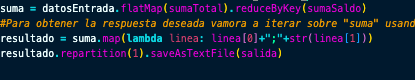
\includegraphics[width=\textwidth, keepaspectratio]{codigo5}
        \caption{Al trabajar con pococs datos, guardamos la salida usando reparittio(1) para guardar la información solamente en una partición y asi evitar la creacion de particiones vacías.}

    \end{figure}
\end{section}
\clearpage
\begin{section}{Ejecución y resultados}
    Para la ejecución del programa, escribimos el siguiente código por la consola de comandos:
    $spark-submit personaGastosSinTarjetaCredito.py file:/Users/adrihp/Master/MBID03/scriptsSpark/Problema1/entrada1 file:/Users/adrihp/Master/MBID03/scriptsSpark/Problema1/salida1$
    
    \vspace{0.25cm}
    Con la entrada:
    \begin{figure}[h]
        \centering
        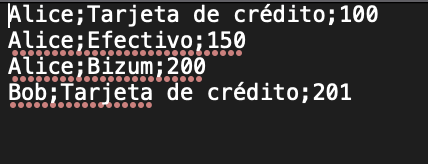
\includegraphics[width=\textwidth, keepaspectratio]{Captura de Pantalla 2022-07-08 a las 13.29.01.png}
    \end{figure}

    La salida que nos devuelve el programa esta guardada en la carpeta salida1/part-00000:
    \begin{figure}[h]
        \centering
        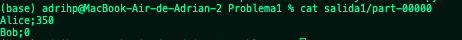
\includegraphics[width=\textwidth, keepaspectratio]{codigo6.png}
    \end{figure}
\end{section}
\end{document}